\chapter{Introdución}
\label{chap:introducion}


\lettrine{E}{n} economía se entiende por venta \textquote{la entrega de un determinado bien o servicio bajo un precio estipulado o convenido y a cambio de una contraprestación económica en forma de dinero por parte de un vendedor o proveedor}~\cite{ventas}. Por lo tanto la realización de ventas supone el núcleo de la actividad económica de un gran margen del espectro económico, donde los actores económicos obtienen ganancias dinerarias tras la entrega de un producto o servicio en el que se especializan. El proceso de venta culmina con la concreción de transacción de venta efectiva ~\cite{proceso-venta}, por lo que una vez realizada dicha transacción es necesario disponer de una herramienta que permita registrar dicha venta, esto es, la relación entre lo que se ha vendido, a quién, cuando y por qué importe.

Con el objetivo de diseñar y desarrollar una herramienta que le permita a una empresa gestionar su catálogo de productos y servicios, así como la cartera de clientes y los produtos y servicios que han contratado dichos clientes a lo largo de su vinculación la empresa nace este trabajo.

Hemos optado por referirnos genéricamente a esta herramienta como un software de gestión de contratación, ya que su principal función es la de gestionar la contratación de los productos ofertados por los distintos clientes de la empresa. Evitamos así el uso del del término más familiar de \acrfull{crm} ya que éste engloba muchas más funcionalidades que las que realiza la herramienta desarrollada: desde un punto de vista informático, un \acrshort{crm} engloba todos los sistemas informáticos de apoyo a la gestión de las relaciones con los clientes, a la venta y al marketing de una empresa, los cuales se integran en los llamados \acrfull{sge}.


\section{Motivación}
\label{sec:motivacion}

El proyecto "Software de gestión de contratación con arquitectura Java EE multicapa para empresas proveedoras de servicios" surge de aunar el deseo de desarrollar una aplicación web como parte del TFG de la titulación y el conocimiento adquirido durante la labor de soporte realizada en un sistema de facturación de una empresa proveedora de servicios.

Visto a muy alto nivel, los procesos de negocio se pueden definir en tres fases tal y como se muestra en la figura ~\ref{fig:fases-proceso-negocio} (página ~\pageref{fig:fases-proceso-negocio}) 


\begin{figure}[hp!]
  \centering
  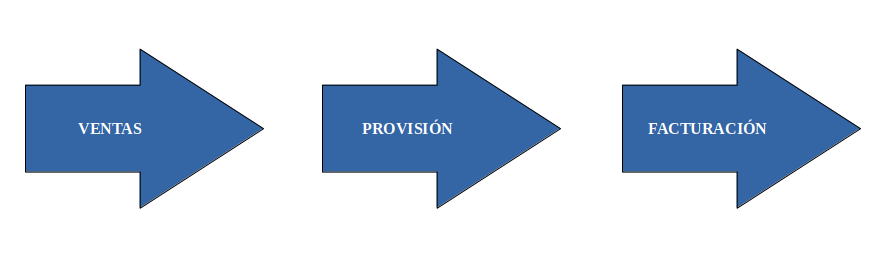
\includegraphics[width=0.50\textwidth]{imaxes/fases-proceso-negocio.png}
  \caption{Fases del proceso de negocio}
  \label{fig:fases-proceso-negocio}
\end{figure}

\begin{itemize}
\item Venta: conjunto de actividades orientadas a realizar y formalizar la venta de un servicio a través de la contratación del mismo.
\item Provisión: conjunto de actividades cuya finalidad es la de proveer el servicio previamente contratado al cliente.
\item Facturación: comprende todas las actividades destinadas a facturar la prestación de los servicios contratados y provisionados y realizar la posterior puesta a cobro de los mismos.
\end{itemize}

Como ya hemos indicado, la herramienta desarrollada para este \acrlong{tfg} se centrará en la fase de venta, concretamente la correspondiente a registrar la venta y gestionar los productos y servicios contratados así como el catálogo de productos y servicios de la empresa.


\section{Definición de objetivos}
\label{sec:objetivos}


El objetivo primordial del presente proyecto es diseñar y desarrollar una aplicación que permita gestionar el catálogo de productos y servicios de una empresa así como la cartera de clientes y sus contrataciones, para lo que se tendrán en cuenta una serie de elementos parametrizables (esto es, modificables según las necesidades del sistema) que conformarán la definición de las entidades a manejar por el sistema.

Además de realizar las diferentes altas, bajas y modificciones de los elementos que comportan el catálogo de productos y servicios y la cartera de clientes, la aplicación desarrollada deberá gestionar el histórico de datos para los elementos susceptibles de cambio y así poder reflejar los continuos cambios derivados que puedan sufrir (cambio de precio en entidades facturables, modificación del servicio contratado, cambios en las tasas impositivas, etc). También permitirá a los usuarios de la misma la gestión de su cuenta, permitiéndoles cambiar tanto la contraseña como los datos de contacto.
La herramienta a desarrollar será una aplicación web con el objetivo de disminuir el riesgo de incompatibilidades y dependencias de software así como de centralizar su distribución y posibles actualizaciones en un único punto.

Durante el desarrollo de este TFG se ha tenido en mente el sector TIC de las operadoras de telefonía, ya que, como se ha indicado anteriormente, se ha querido aprovechar el conocimiento adquirido a través de la experiencia profesional, aunque podría adaptarse a cualquier otra empresa con necesidades similares.

